\subsection{MSVC: x86}

\lstinputlisting{patterns/04_scanf/2_global/ex2_MSVC.asm}

Nesse caso, a variável \TT{x} é definida no segmento \TT{\_DATA} e nenhuma memória é alocada na pilha local.
Ela é acessada diretamente, não através da pilha.
Variáveis globais não inicialiadas não ocupam espaço no arquivo executável 
(realmente, ninguém precisa alocar espaço para uma variável inicialmente valendo zero), 
mas quando alguém acessa o endereço delas, o sistema operacional vai alocar um bloco contendo somente zeros nele.
\footnote{\ac{TBT}: That is how a \ac{VM} behaves}.

Agora vamos definir um valor para a variável:

% TODO translate
\lstinputlisting{patterns/04_scanf/2_global/default_value_EN.c}

Nós temos:

\begin{lstlisting}
_DATA	SEGMENT
_x	DD	0aH

...
\end{lstlisting}

Aqui nós vemos um valor \TT{0xA} do tipo DWORD (DD significa DWORD = 32 bits) para essa variável.

Se você abrir o .exe compilado no \IDA, você pode ver a variável \IT{x} colocada no começo do segmento \TT{\_DATA},
e depois disso você pode ver as strings.

Se você abrir o .exe compilado no exemplo anterior no \IDA, onde o valor de x não foi declarado, você poderá ver algo assim:

\begin{lstlisting}
.data:0040FA80 _x              dd ?                    ; DATA XREF: _main+10
.data:0040FA80                                         ; _main+22
.data:0040FA84 dword_40FA84    dd ?                    ; DATA XREF: _memset+1E
.data:0040FA84                                         ; unknown_libname_1+28
.data:0040FA88 dword_40FA88    dd ?                    ; DATA XREF: ___sbh_find_block+5
.data:0040FA88                                         ; ___sbh_free_block+2BC
.data:0040FA8C ; LPVOID lpMem
.data:0040FA8C lpMem           dd ?                    ; DATA XREF: ___sbh_find_block+B
.data:0040FA8C                                         ; ___sbh_free_block+2CA
.data:0040FA90 dword_40FA90    dd ?                    ; DATA XREF: _V6_HeapAlloc+13
.data:0040FA90                                         ; __calloc_impl+72
.data:0040FA94 dword_40FA94    dd ?                    ; DATA XREF: ___sbh_free_block+2FE
\end{lstlisting}

\TT{\_x} está marcada com \TT{?} juntamente com o resto das variáveis que não precisam ser inicializadas.
Isso implica que após carregar o .exe para a memória, um espaço para todas essas variáveis será alocado e preenchido com zeros \cite[6.7.8p10]{C99TC3}.
Mas no arquivo .exe essas variáveis não inicializadas não ocupam nenhum espaço.
Isso é conveniente para arrays grandes, por exemplo.

\EN{\clearpage
\subsection{MSVC: x86 + \olly}
\myindex{\olly}

Things are even simpler here:

\begin{figure}[H]
\centering
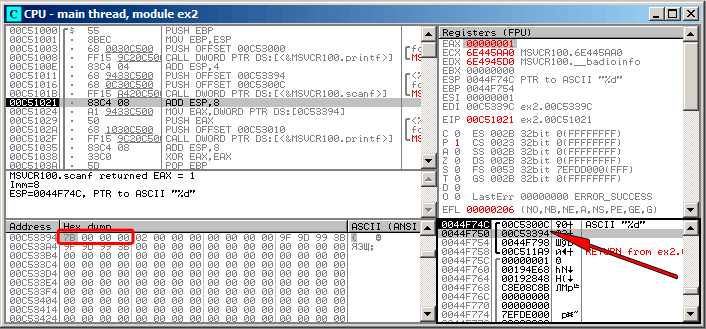
\includegraphics[scale=\FigScale]{patterns/04_scanf/2_global/ex2_olly_1.png}
\caption{\olly: after \scanf execution}
\label{fig:scanf_ex2_olly_1}
\end{figure}

The variable is located in the data segment.
After the \PUSH instruction (pushing the address of $x$) gets executed, 
the address appears in the stack window. Right-click on that row and select \q{Follow in dump}.
The variable will appear in the memory window on the left.
After we have entered 123 in the console, 
\TT{0x7B} appears in the memory window (see the highlighted screenshot regions).

But why is the first byte \TT{7B}?
Thinking logically, \TT{00 00 00 7B} should be
there.
The cause for this is referred as  \gls{endianness}, and x86 uses \IT{little-endian}.
This implies that the lowest byte is written first, and the highest written last.
Read more about it at: \myref{sec:endianness}.
Back to the example, the 32-bit value is loaded from this memory address into \EAX and passed to \printf.

The memory address of $x$ is \TT{0x00C53394}.

\clearpage
In \olly we can review the process memory map (Alt-M)
and we can see that this address is inside the \TT{.data} PE-segment of our program:

\begin{figure}[H]
\centering
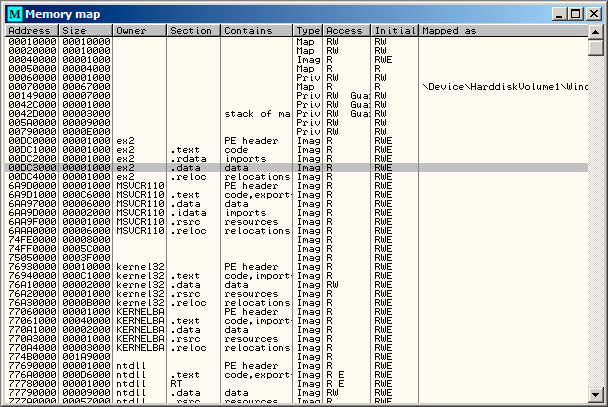
\includegraphics[scale=\FigScale]{patterns/04_scanf/2_global/ex2_olly_2.png}
\caption{\olly: process memory map}
\label{fig:scanf_ex2_olly_2}
\end{figure}

}
\RU{\clearpage
\subsectionold{MSVC: x86 + \olly}
\myindex{\olly}

Тут даже проще:

\begin{figure}[H]
\centering
\myincludegraphics{patterns/04_scanf/2_global/ex2_olly_1.png}
\caption{\olly: после исполнения \scanf}
\label{fig:scanf_ex2_olly_1}
\end{figure}

Переменная хранится в сегменте данных.
Кстати, после исполнения инструкции \PUSH (заталкивающей адрес $x$) адрес появится в стеке, 
и на этом элементе можно нажать правой кнопкой, выбрать \q{Follow in dump}.
И в окне памяти слева появится эта переменная.

После того как в консоли введем 123, здесь появится \TT{0x7B}.

Почему самый первый байт это \TT{7B}?
По логике вещей, здесь должно было бы быть \TT{00 00 00 7B}.
Это называется \gls{endianness}, и в x86 принят формат \IT{little-endian}.
Это означает, что в начале записывается самый младший байт, а заканчивается самым старшим байтом.
Больше об этом: \myref{sec:endianness}.

Позже из этого места в памяти 32-битное значение загружается в \EAX и передается в \printf.

Адрес переменной $x$ в памяти \TT{0x00C53394}.

\clearpage
В \olly{} мы можем посмотреть карту памяти процесса (Alt-M) и увидим, что этот адрес
внутри PE-сегмента \TT{.data} нашей программы:

\begin{figure}[H]
\centering
\myincludegraphics{patterns/04_scanf/2_global/ex2_olly_2.png}
\caption{\olly: карта памяти процесса}
\label{fig:scanf_ex2_olly_2}
\end{figure}
}
\ITA{\clearpage
\subsectionold{MSVC: x86 + \olly}
\myindex{\olly}

Il quadro qui è ancora più semplice:

\begin{figure}[H]
\centering
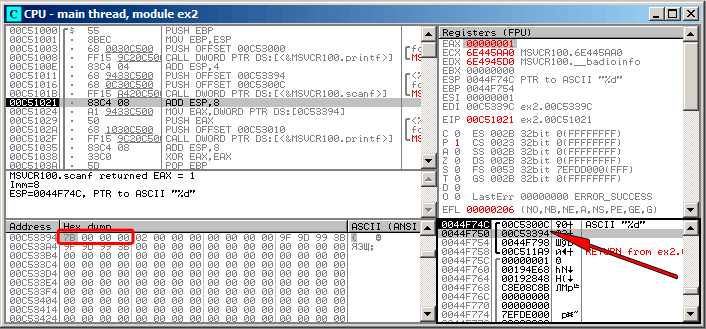
\includegraphics[scale=\FigScale]{patterns/04_scanf/2_global/ex2_olly_1.png}
\caption{\olly: after \scanf execution}
\label{fig:scanf_ex2_olly_1}
\end{figure}

La variabile è collocata nel data segment.
Dopo che l'istruzione \PUSH (che fa il push dell'indirizzo di $x$) viene eseguita, 
l'indirizzo appare nella finestra dello stack. Facciamo click destro su quella riga e selezioniamo \q{Follow in dump}.
La variabile apparirà nella finestra di memoria a sinistra.
Dopo aver inserito il valore 123 in console, 
\TT{0x7B} apparirà nella finestra della memoria (vedere regioni evidenziate nello screenshot).

Ma perchè il primo byte è \TT{7B}?
A rigor di logica, dovremmo trovare \TT{00 00 00 7B}.
La causa per cui troviamo invece \TT{7B} è detta \gls{endianness}, e x86 usa la convenzione \IT{little-endian}.
Ciò significa che il byte piu basso è scritto per primo, e quello più alto per ultimo.
Maggiori informazioni sono disponibili nella sezione: \myref{sec:endianness}.
Tornando all'esempio, il valore a 32-bit è caricato da questo indirizzo di memoria in \EAX e passato a \printf.

L'indirizzo in memoria di $x$ è \TT{0x00C53394}.

\clearpage
In \olly possiamo osservare la mappa di memoria di un processo  (process memory map, Alt-M)
e notare che questo indirizzo è dentro il segmento PE \TT{.data} del nostro programma:

\begin{figure}[H]
\centering
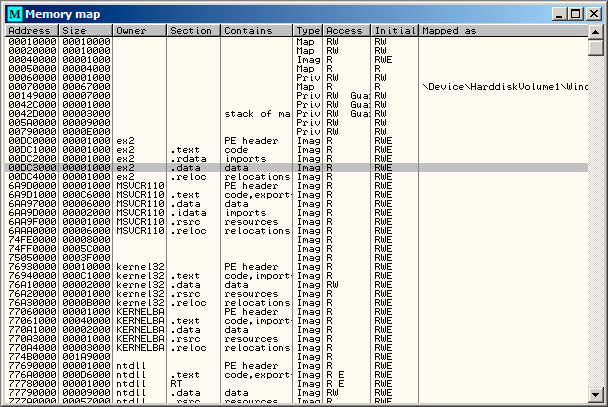
\includegraphics[scale=\FigScale]{patterns/04_scanf/2_global/ex2_olly_2.png}
\caption{\olly: process memory map}
\label{fig:scanf_ex2_olly_2}
\end{figure}

}


\subsection{GCC: x86}

\PTBRph{}

\subsection{MSVC: x64}

% TODO translate
\lstinputlisting[caption=MSVC 2012 x64]{patterns/04_scanf/2_global/ex2_MSVC_x64_EN.asm}

O código é quase o mesmo que no x86.
Por favor, perceba que o endereço da variável x é passado para \TT{scanf()} usando uma instrução \LEA,
enquanto os valores das variáveis são passadas para o segundo \printf usando uma instrução \MOV.
\TT{DWORD PTR} é uma parte da linguagem assembly (sem relação com o código de máquina),
indicando que o tamanho da informação da variável é de 32-bits e que a instrução \MOV tem de ser codificada de acordo.

